%-----------------------------------------------
% Dateiname: Thesis.tex
% Autor    : Stefano Kowalke <blueduck@gmx.net>
% Lizenz   : BSD
%-----------------------------------------------

%-------------------------
% Importiere die Präambel
%-------------------------
%-----------------------------------------------
% Dateiname: Thesis-Preamble.tex
% Autor    : Stefano Kowalke <blueduck@gmx.net>
% Lizenz   : BSD
%-----------------------------------------------

%----------------------------------
% Dokumentenklasse DINA4 einseitig
%----------------------------------
\documentclass[
	fontsize    = 11pt,           % Die Schriftgröße
	twoside     = false,          % scrbook hat per Default ein Zwei-Seitenlayout
	parskip     = full,           % Steuert die Absätze. http://www.rrzn.uni-hannover.de/fileadmin/kurse/material/latex/scrguide.pdf Tabelle 3.7
	headsepline,                  % Fügt eine Trennungslinie in den Seitenkopf
	footnotes   = multiple,       % Fügt ein Komma zwischen den Indexzahlen bei aufeinanderfolgende Fußnoten ein
	numbers     = noendperiod     % Keinen Punkt der letzten Gliederungsebene in der Überschrift  -> 1.2.1 statt 1.2.1.
]{scrbook}

%\includeonly{Chapters/Doctrine}
\PassOptionsToPackage{
    %layout,
    drafting,
    eulerchapternumbers,
    eulermath,
    colophon,
    bettertable,
    %minionpro,
    %dottedtoc,
}{thesis}


%===============
% Pakete laden
%===============
\usepackage{fontspec}                      % Wird von LuLaTeX benöigt und löst "fontenc" ab.
\usepackage{polyglossia}                   % Wird von LuLaTeX benöigt und löst "babel" ab.
\usepackage[german=quotes]{csquotes}       % Anführungszeichen global im Dokument steuern. Paket wird von "polyglossia" empfohlen.

\usepackage[
	backend=biber,                         % Benutzer biber zur Erstellung
	bibwarn=true,                          % Warne, wenn das BiTex Format falsch ist
	autolang=other,
	style=alphabetic-verb,
	bibstyle=alphabetic-verb,
]
{biblatex}                                 % Nutze Biblatex zur Erstellung des Literaturverzeichnis
\addbibresource{Bib/Bibliography.bib}      % Die Literatureinträge
\usepackage{minted}                        % Sourcecode Highlighting. Dieses Package benötigt Python und Pygments 1.5. Version 1.6 macht Probleme mit gerade Anführungszeichen (') - es stellt sie als normale Anführungszeichen dar.
\usepackage[punct-after=true]{fnpct}       % Ermöglicht das Setzen der Indexzahlen der Fußnoten hinter dem Punkt oder Komma. Hier ist es dafür gedacht die Option footnotes=multiple von KOMA wiederherzustellen, die durch das Hyperref Paket kaputt gegangen ist.
\usepackage{hyperref}                      % Stellt Links in Schreibmaschinenschrift dar und legt einen Link über den Text.
                                           % Dieses Package sollte als letztes aufgerufen werden, da es Problem mit Anderen geben könnte
\usepackage[
    xindy={language=german,codepage=din5007-utf8}, % Ruft Xindy zum Erstellen des Index in der deutschen Version auf
    toc,                                   % Fügt die Glossare dem Inhaltsverzeichnis zu
    acronym,                               % Erstellt ein neues Glossar mit dem Label "acronym"
    nonumberlist,                          % Fügt die Seitenzahlen hinzu, auf denen der Eintrag vorkommt, nicht hinzu
    nopostdot                              % Entferne den Punkt am Ende der Definition
    ]{glossaries}                          % Erstellt Glossar und Abkürzungsverzeichnis. Laut der Dokumentation ist es ausdrücklich notwendig, dass es nach dem Package hyperref eingebunden werden muß
\makeglossaries                            % Anweisung das Glossar zu erstellen

\newfontfamily\quotefont[Ligatures=TeX]{Palatino} % The font for the quotation marks at a quote

\usepackage{chronosys} % Creates timelines

%=================================================
% Angaben zur Arbeit wie Titel und Name des Autor
%=================================================
\newcommand{\myTitle}{Integration der Datenbank-Abstraktionsschicht Doctrine2\xspace}
\newcommand{\myTitleSecondLine}{in das Content-Management-System TYPO3\xspace}
%\newcommand{\mySubtitle}{Put your subtitle here\xspace}
%\newcommand{\myDegree}{Put your degree here\xspace}
\newcommand{\myName}{Stefan Kowalke\xspace}
\newcommand{\myEMail}{<stefan.kowalke@stud.fh-flensburg.de>\xspace}
\newcommand{\myMatricleNumber}{485366\xspace}
\newcommand{\myProf}{Prof. Dr. Hans-Werner Lang\xspace}
\newcommand{\myOtherProf}{Dipl. VK Tobias Hiep\xspace}
%\newcommand{\mySupervisor}{Put name here\xspace}
\newcommand{\myUni}{\uppercase{\large Fachhochschule Flensburg}\xspace}
\newcommand{\myDepartment}{Angewandte Informatik\xspace}
%\newcommand{\myFaculty}{Put data here\xspace}
\newcommand{\myMajor}{Medieninformatik\xspace}
\newcommand{\myLocation}{Flensburg\xspace}
\newcommand{\myTime}{März 2014\xspace}
%\newcommand{\myVersion}{version 4.1\xspace}


%----------------
% Renew commands
%----------------
%\renewcommand*{\multfootsep}{,\nobreakspace}  % Fügt bei den hochgestellten Indexzahlen von Fußnoten ein Leerzeichen nach dem Komma ein
\deffootnote{1em}{1em}{\thefootnotemark\ }    % Setzt die Indexzahlen in den Fußnoten etwas entfernt vom Text

%---------------------------------------------------------------
% Renew the citation style from parenthesis to square brackets:
%---------------------------------------------------------------
% (Popel 2007, S. 59–63) -> [Popel 2007, S. 59–63]
% http://tex.stackexchange.com/questions/16765/biblatex-author-year-square-brackets
%---------------------------------------------------------------
\makeatletter
\newrobustcmd*{\parentexttrack}[1]{%
  \begingroup
  \blx@blxinit
  \blx@setsfcodes
  \blx@bibopenparen#1\blx@bibcloseparen
  \endgroup}

\AtEveryCite{%
  \let\parentext=\parentexttrack%
  \let\bibopenparen=\bibopenbracket%
  \let\bibcloseparen=\bibclosebracket}
\makeatother

%----------------------
% Neue Quoting Umgebung
%----------------------
\newcommand*\quotesize{60} % if quote size changes, need a way to make shifts relative
% Make commands for the quotes
\newcommand*{\openquote}
   {\tikz[remember picture,overlay,xshift=-4ex,yshift=-2.5ex]
   \node (OQ) {\quotefont\fontsize{\quotesize}{\quotesize}\selectfont``};\kern0pt}

\newcommand*{\closequote}[1]
  {\tikz[remember picture,overlay,xshift=4ex,yshift={#1}]
   \node (CQ) {\quotefont\fontsize{\quotesize}{\quotesize}\selectfont''};}

% select a colour for the shading
\definecolor{shadecolor}{gray}{0.95}

\newcommand*\shadedauthorformat{\emph} % define format for the author argument

% Now a command to allow left, right and centre alignment of the author
\newcommand*\authoralign[1]{%
  \if#1l
    \def\authorfill{}\def\quotefill{\hfill}
  \else
    \if#1r
      \def\authorfill{\hfill}\def\quotefill{}
    \else
      \if#1c
        \gdef\authorfill{\hfill}\def\quotefill{\hfill}
      \else\typeout{Invalid option}
      \fi
    \fi
  \fi}

% wrap everything in its own environment which takes one argument (autor) and one 
% optional argument [l, c or r]
\newenvironment{shadequote}[2][l]%
{\authoralign{#1}
\ifblank{#2}
   {\def\shadequoteauthor{}\def\yshift{-2ex}\def\quotefill{\hfill}}
   {\def\shadequoteauthor{\par\authorfill\shadedauthorformat{#2}}\def\yshift{2ex}}
\begin{snugshade}\begin{quote}\openquote}
{\shadequoteauthor\quotefill\interlinepenalty=10000\end{quote}\end{snugshade}}

%------------------
% Eigene Kommandos
%------------------


%---------------------
% Spracheinstellungen
%---------------------
\setdefaultlanguage[spelling=new]{german}   % Die Sprache muß vor dem Einbinden von dem Blindtextpackage eingestellt werden
\usepackage{blindtext}                      % Erstellt schnell und einfach Blindtexte mit \Blindtext. Wird ausnahmsweise hier eingebunden


%-------------------
% Linkkonfiguration
%-------------------
\hypersetup
{
	pdftitle       = {\myTitle \myTitleSecondLine},
	pdfauthor      = {\myName},
	pdfsubject     = {\myTitle \myTitleSecondLine},
	pdfcreator     = {\myName},
	pdfkeywords    = {typo3} {dbal} {doctrine} {mysql} {postgres},
	linktoc        = all,
	colorlinks     = true,
	linkcolor      = black,
	citecolor      = black,
	filecolor      = black,
	urlcolor       = blue,
}

%----------
% Grafiken
%----------
\graphicspath{ {gfx/} }

%--------------
% Code Listing
%--------------
%**************************************
% Schrifteinstellungen für Codelistings
%
\setmonofont[Scale=0.75]{Source Code Pro Light}
\definecolor{bg}{rgb}{0.95,0.95,0.95}
\newminted{php}{
	linenos              = true,
	xleftmargin          = 2em,
	tabsize              = 4,
	bgcolor              = bg,
	funcnamehighlighting = true
}

\newminted{mysql}{
	linenos     = true,
	bgcolor     = bg,
	xleftmargin = 2em
}

\usepackage{thesis}


%--------------------------------
% Importiere die Glossareinträge
%--------------------------------
%-----------------------------------------------
% Dateiname: Definitions.tex
% Autor    : Stefano Kowalke <blueduck@gmx.net>
% Lizenz   : BSD
%-----------------------------------------------

%-----------------
% Abkürzungen
%-----------------
% http://tex.stackexchange.com/questions/8946/how-to-combine-acronym-and-glossary
\newacronym{ide}{IDE}{Integrated Development Environment}
\newacronym{cgl}{CGL}{Coding Guidelines}
\newacronym{sql}{SQL}{Structured Query Language}
\newacronym{dbms}{DBMS}{Database Management System}
\newacronym{jdo}{JDO}{Java Data Objects}
\newacronym{pdo}{PDO}{PHP Data Objects}
\newacronym{ter}{TER}{TYPO3 Extension Repository}
\newacronym{em}{EM}{Extension Manager}
\newacronym{php}{PHP}{PHP: Hypertext Processor}
\newacronym{fe}{FE}{Frontend}
\newacronym{be}{BE}{Backend}
\newacronym{tca}{TCA}{Table Content Array\protect\glsadd{glos:tca}}
%\newacronym{dbal}{DBAL}{Database Abstraction Layer\protect\glsadd{glos:dbal}}
\newacronym{dbal}{DBAL}{Database Abstraction Layer}
\newacronym{cms}{CMS}{Content Management-System}
\newacronym{cmf}{CMF}{Content Management-Framework}
\newacronym{ecms}{ECMS}{Enterprise Content Management-System}
\newacronym{wcms}{WCMS}{Web Content Management-System}
\newacronym{orm}{ORM}{Object-relational mapping}
\newacronym{jcr}{JCR}{Content Repository for Java Technology API}
\newacronym{mvc}{MVC}{Model-View-Controller}
\newacronym{api}{API}{Application Programming Interface}
\newacronym{gpl2}{GPL2}{GNU General Public License v.2}

\newglossaryentry{t3assoc}
{
	type=\acronymtype,
	name={T3Assoc},
	description={TYPO3 Association},
	first={TYPO3 Association (T3Assoc)}
}

%-------------
% glossareinträge
%-------------
\newglossaryentry{glos:dbal}
{
	name={dbal},
	description={a very long description of of what is dbal}
}

\newglossaryentry{glos:tca}
{
	name={TCA},
	description={Das TCA ist ein globales PHP Array, welches die Definition von Datanbanktabellen weit über die Möglichkeiten herkömmlichen SQLs erweitert. Seine Hauptaufgabe besteht in der Definition der, durch das TYPO3 CMS Backend, editierbaren Tabellen. Es beschreibt die Beziehungen zu anderen Tabellen, welches Feld einer Tabelle soll in welchen Layout im \gls{be} dargestellt werden und wie soll das Feld validiert werden. Enthält eine Tabelle keinen Eintrag im TCA ist sie im Backend nicht sichtbar.}
}

\newglossaryentry{composer}
{
	name={Composer},
	description={Composer ist ein Dependency Manager\footnote{https://getcomposer.org/} für PHP, welcher von der Kommandozeile aufgerufen wird. Es dient zum Auflösen von Abhängigkeiten eines Projektes. Diese Abhängigkeiten werden in einer \pdf{composer.json}-Datei definiert und durch Ausführung des Programms in Verbindung mit der Konfigurationsdatei in dem Ordner \pdf{vendor} installiert.}
}

\newglossaryentry{glos:sqlDialect}
{
	name={SQL-Dialekt},
	description={Als SQL Dialekt wird ein vom SQL-Standard abweichender Hersteller-spezifischer Sprachumfang bezeichnet. Ein Dialekt ist in der Regel kompatibel mit dem Standard und erweitert ihn um eigene Sprachkonstrukte.}
}

\newglossaryentry{glos:adaptee}
{
	name={Adaptee},
	description={Eine Klasse die vone eine Adapterklasse in eine andere Klasse konvertiert wird.}
}

\newglossaryentry{glos:extkey}
{
	name={Extension-Key},
	description={Ein einmaliger Bezeichner für den internen Namen einer TYPO3 CMS Extension.}
}


%--------------------------------------
% Hier fängt der eigentliche Inhalt an
%--------------------------------------
\begin{document}
	\frontmatter
		%-----------------------------------------------
% Dateiname: Titlepage.tex
% Autor    : Stefano Kowalke <blueduck@gmx.net>
% Lizenz   : BSD
%-----------------------------------------------
\begin{titlepage}
	\begin{center}
		\myUni\\
	\end{center}
	\begin{center}
		\large Fachbereich \myDepartment
	\end{center}
	\begin{verbatim}


	\end{verbatim}
	\begin{center}
		\uppercase{\textbf{\large Bachelorthesis}}
	\end{center}
	\begin{verbatim}
	\end{verbatim}
	\begin{center}
		\textbf{im Studiengang \myMajor}
	\end{center}
	\begin{verbatim}







	\end{verbatim}
	\begin{flushleft}
		\begin{tabular}{lll}
			\textbf{Thema:} & & \myTitle \\
			&&  \myTitleSecondLine \\
			& & \\
			& & \\
			& & \\
			\textbf{eingereicht von:} & & \myName\ \myEMail\\
			& & \\
			& & \\
			\textbf{Matrikelnummer:} & & \myMatricleNumber\\
			& & \\
			& & \\
			\textbf{Abgabedatum:} & & \today\\
			& & \\
			& & \\
			\textbf{Erstprüfer:} & & \myProf\\
			& & \\
			& & \\
			\textbf{Zweitprüfer:} & & \myOtherProf
		\end{tabular}
	\end{flushleft}
\end{titlepage}

		%-----------------------------------------------
% Dateiname: Colophon.tex
% Autor    : Stefano Kowalke <blueduck@gmx.net>
% Lizenz   : BSD
%-----------------------------------------------
\thispagestyle{empty}
\vspace*{\fill}
\begin{flushleft}
    \sffamily
    \footnotesize
    \noindent
Dieses Dokument wurde am \today\ mit \InfoLaTeX\ gesetzt.
    \par\bigskip\noindent
    \begin{tabular}{ll}
Schrift: & \textcolor{red}{12pt-TODO}\\
Typographie: & \KOMAScriptVersion\\
System: & \InfoTeX\ auf OSX 10.8\\
Editor: & Mou 0.8.5 beta und VIM 7.4 \\
    \end{tabular}
    \par\bigskip\noindent
    \textcolor{red}{Die Dokumentenvorlage ist unter TODO frei verfügbar}
\end{flushleft}
\normalsize

		%-----------------------------------------------
% Dateiname: Abstract.tex
% Autor    : Stefano Kowalke <blueduck@gmx.net>
% Lizenz   : BSD
%-----------------------------------------------
%\renewcommand{\abstractname}{Abstract}
\pdfbookmark[1]{Abstract}{Abstract}
\begingroup
\let\clearpage\relax
\let\cleardoublepage\relax
\let\cleardoublepage\relax

\chapter*{Abstract}
\label{ch:abstractEn}
Web applications are often developed around one particular database management system. In the past MySQL was used a lot. To decouple the web application from this dependency you could use the database abstraction layer PDO, which is bundled with PHP. Doctrine DBAL goes one step further which offers, based on PDO, a unified interface to a broad range of other database management systems. Additionally Doctrine DBAL is the base of Doctrine ORM – a framework for object-relational database mapping, which is used by TYPO3 Flow and TYPO3 Neos. This paper demonstrates how to decouple the dependency to MySQL by integrating Doctrine DBAL into the content manangement system TYPO3 CMS. On top of that it implements an abstract query language for the underlying database with a transparent use of Prepared Statements.

\vfill

\chapter{Zusammenfassung}
\label{ch:abstractDe}
Webanwendungen werden häufig um ein Datenbankmanagementsystem herum entworfen. In der Vergangenheit war dies oft MySQL. Um eine Webanwendung aus der Abhängigkeit zu einem spezifischen Datenbankmanagementsystem zu lösen, kann die, von PHP mitgelieferte, Datenbankabstraktionsschicht PDO genutzt werden. Einen Schritt weiter geht Doctrine DBAL, welches – auf PDO aufbauend – eine einheitliche Schnittstelle zu weiteren Datenbankmanagementsystemen bereitstellt. Doctrine DBAL ist zudem die Grundlage für Doctrine ORM - ein Framework zur objektrelationalen Abbildung von Objekten auf eine Datenbank, das in TYPO3 Flow und TYPO3 Neos eingesetzt wird. Diese Arbeit demonstriert, wie durch die Integration von Doctrine DBAL in das Content-Manangement-System TYPO3 CMS die Abhängigkeit zu MySQL entfernt werden kann. Zusätzlich wird eine abstrakte Abfragesprache für die zugrundeliegende Datenbank eingeführt, die eine transparente Nutzung von Prepared Statements anbietet.

\endgroup
\vfill

		\newpage
		\thispagestyle{empty}
		\hspace{1cm}
		\newpage
		\thispagestyle{empty}
		\vspace*{\fill}
		\begin{verse}
			\centering
			``'The Babel fish,' said The Hitchhiker's Guide to the Galaxy quietly, 'is small, yellow and leech-like, and probably the oddest thing in the Universe.\\
			...\\
			The practical upshot of all this is that if you stick a Babel fish in your ear you can instantly understand anything in any form of language.'''

			– Douglas Adams, The Hitchhiker's Guide to the Galaxy
			%``War is peace.\\
			%Freedom is slavery.\\
			%Ignorance is strength.''

			%– George Orwell, 1984
		\end{verse}
		%\begin{quote}
			%\hfill ``@WilliamShatner Yes, Standard Orbit, Captain. And we're detecting signs of life on the surface.''\\
			%\\
			%\hfill – William Shatner und ISS Commander Chris Hadfield am 03.01.2013 auf Twitter (\url{https://twitter.com/Cmdr_Hadfield/status/286948264236945408})
		%\end{quote}
		%\begin{quote}
			%\hfill ``'The Answer to the Great Question\ldots~Of Life, the Universe and Everything\ldots~Is\ldots~Forty-two,' said Deep Thought, with infinite majesty and calm.''\\
			%\\
			%\hfill – Douglas Adams, The Hitchhiker's Guide to the Galaxy

		%\end{quote}
		\vspace*{\fill}
		\newpage
		\tableofcontents
	\mainmatter
		%-----------------------------------------------
% Dateiname: Introduction.tex
% Autor    : Stefano Kowalke <blueduck@gmx.net>
% Lizenz   : BSD
%-----------------------------------------------
\chapter{Einleitung}
\label{ch:intro}
Als sich auf den Developer Days 2006 das Entwicklerteam für einen Nachfolger der eben erst erschienen \gls{cms} TYPO3 Version 4.0 formierte[News T3Org], war wohl keinem der dort Anwesenden klar wohin die Reise gehen würde – ging man anfänglich noch von einem Restrukturierung (engl. Refactoring) der schon vorhandenen Codebasis aus.

In der Konzeptionsphase kristallisierte sich immer mehr heraus, dass es damit nicht getan sein würde. Der Nachfolger mit dem Arbeitstitel ``Phoenix'' sollte nicht nur den zukünftigen Anforderungen des Web standhalten, sondern die Position der Version 4.0 weiter ausbauen. Das Entwicklerteam um Chefentwickler Robert Lemke entschloss sich die Version 5.0 des Systems komplett neu zu schreiben [Quelle anfügen] und merkte dabei, dass Entwickler bei der Programmierung von Webanwendungen immer wieder mit den gleichen Problemen wie Routing, die Erstellung und Validierung von Formularen, Login von Benutzern oder dem Aufbau einer Verbindung zur Datenbank konfrontiert werden.

Die Idee eines – von dem Content-Management-System – unabhängigen PHP Frameworks war geboren und wurde zunächst auf den Namen FLOW3 getauft. Dieses Framework sollte die spätere Basis für TYPO3 5.0 bilden und all die oben beispielhaft angeführten wiederkehrenden Aufgaben übernehmen. Die Version 5.0 von TYPO3 sollte lediglich eins von vielen Packages darstellen mit denen FLOW3 erweitert werden kann. Vielmehr wurde es als eigenständiges ``Webapplication Framework'' konzipiert und umgesetzt, so dass es auch ohne ein \gls{cms} betrieben werden kann und auch wird. [Quelle zu Rossmann einfügen].

Schon in einer recht frühen Entwicklungsphase hat man sich dem Thema Persistenz gewidmet, die zunächst noch als ``\gls{jcr}'' in PHP implementiert [Quelle einfügen], jedoch später wegen zu vieler Probleme bei der Portierung der Java Spezifikation JSR-170 [stimmt die Nummer?] nach PHP [Quelle Blogeintrag von Karsten] durch eine eigene Persistenzschicht ersetzt wurde. Im weiteren Verlauf der Entwicklung kam man von dieser Idee wieder ab, da das Bereitstellen und die Pflege einer eigenen Datenbankschnittstelle zu aufwändig sei und andere Projekte wie Doctrine oder Propel schon fertige Lösungen anboten. Schlußendlich entschied man sich für die Integration von Doctrine als Persistenzschicht. [Quellen zu Github einfügen]

Für die Anwender stellt sich bei einem Versionssprung stets die Frage, ob eine Migration von der alten zur neuen Version möglich ist und mit wieviel Aufwand dies verbunden sein würde. Diesen Bedenken folgend trafen sich die Kernentwickler beider Teams 2008 in Berlin, um die Routemaps beider Projekte in Einklang zu bringen. Als ein Ergebnis dieses Treffens wurde das ``Berlin Manifesto'' [Quelle angeben] bekanntgegeben, welches mit kappen Worten feststellt\footnote{Mittlerweile wird TYPO3 Neos innerhalb der Community nicht mehr als der Nachfolger von TYPO3 \gls{cms} angesehen. Es stellt lediglich – wie TYPO3 Flow – ein weiteres Produkt innerhalb der TYPO3 Familie dar. [Quellen angabe]}
:
\begin{shadequote}[l]{Die TYPO3 Kernentwickler}
	\begin{itemize}
		\item TYPO3 v4 continues to be actively developed
		\item v4 development will continue after the the release of v5
		\item Future releases of v4 will see its features converge with those in TYPO3 v5
		\item TYPO3 v5 will be the successor to TYPO3 v4
		\item Migration of content from TYPO3 v4 to TYPO3 v5 will be easily possible
		\item TYPO3 v5 will introduce many new concepts and ideas. Learning never stops and we'll help with adequate resources to ensure a smooth transition
	\end{itemize}
\end{shadequote}

An der Umsetzung wurde sofort nach dem Treffen begonnen, indem Teile des FLOW3 Frameworks nach TYPO3 Version 4.0 zurück portiert und unter dem Namen \emph{Extbase} als Extension veröffentlicht wurden. Es erfüllt zu gleichen Teilen die Punkte 3 und 6 des Manifests, da es die neuen Konzepte aus FLOW3 der Version 4.0 zur Verfügung stellt und somit gleichzeitig diese Version näher an die Technologie des Frameworks heranführt.

Die Aufgabe von Extbase besteht darin ein \gls{api} bereitzustellen, mit denen Entwickler von Extensions auf die internen Ressourcen und Funktionen von TYPO3 \gls{cms} zugreifen und das System somit nach eigenen Wünschen und Anforderungen erweitern können, ohne den Code des \gls{cms} selbst verändern zu müssen. Es ist als vollständiger Ersatz der bis dahin angebotenen PI-Base \gls{api} [LINK ZU PI BASE] konzipiert worden, wobei es aktuell noch möglich ist sich für einen der beiden Ansätze zu entscheiden.

Extbase führt per Definition einige – bis dahin in TYPO3 v4 unbekannte – Programmierparadigmen ein. Als größter Unterschied zu dem PI-Based Ansatz ist hier sicherlich das \gls{mvc} Pattern zu nennen. Dabei werden die Daten im Model vorgehalten, der View gibt die Daten aus und der Controller steuert die Ausgabe der Daten. Das Model ist unabhängig von der View, was bedeutet, dass die gleichen Daten auf verschiedene Weise ausgegeben werden können. Man denke hier an Meßdaten, die zum einen als Tabelle über einer Listview dargestellt werden können oder als Diagramme mit einer entsprechenden View.

Das Model – eine herkömmliche PHP Klasse – wird dabei von Extbase automatisch auf die Datenbank abgebildet, so dass ein Objekt eine Zeile darstellt und dessen Eigenschaften als Spalten der Tabelle interpretiert werden. Diese Technik wird als Objektrelationale Abbildung (engl. \gls{orm}) genannt. Das zum Einsatz kommende \gls{orm} ist Bestandteil der oben erwähnten selbstgeschriebenen Persistenzschicht von FLOW3, da Extbase zu der Zeit rückportiert wurde, als diese bei FLOW3 im Einsatz war.

Obwohl Extbase beständig weiterentwickelt wird und es der Wunsch der Community ist, die in darin verwendete Persistenzschicht gegen Doctrine 2 auszutauschen, was sich in Form von Posts auf der Mailingliste [Ausdruck und Link der Quelle einfügen] oder in Prototypen ausdrückt [Link der Quelle einfügen], ist dies bis heute noch nicht realisiert worden. Der Chefentwickler von Doctrine, Benjamin Eberlei, hat gegenüber dem Autor in einer persönlichen Korrespondenz die unterschiedlichen Ansätze beider Projekte wie folgt zum Ausdruck gebracht:
\begin{shadequote}{Benjamin Eberlei per E-Mail vom 17.12.13 00:12}
	(\ldots) Doctrine nutzt das Collection interface, Extbase SplObjectStorage.Doctrine Associationen funktionieren semantisch anders als in Extbase, z.B. Inverse/Owning Side Requirements.
	Typo3 hat die Enabled/Deleted flags an m\_n tabellen, sowie das start\_date Konzept. Das gibts in Doctrine \gls{orm} alles evtl nur über Filter \gls{api}, aber vermutlich nicht vollständig abbildbar.
	Das betrifft aber alles nur das \gls{orm}, das Doctrine \gls{dbal} hinter Extbase zu setzen ist ein ganz anderes Abstraktionslevel.
\end{shadequote}
[Email in Literatur anhängen und als Quelle anfügen]

Zum jetzigen Zeitpunkt wird die \gls{dbal} in TYPO3 durch eine Systemextension [Glossareintrag] bereitstellt, die auf der externen Bibliothek AdoDB basiert, welche jedoch Anzeichen des Stillstands aufzeigt und davon ausgegangen werden kann, dass das Projekt nicht weiterentwickelt wird. [Linkt zu SourceForge]

Anhand dieser Fakten wird ersichtlich, dass die Integration von Doctrine erstrebenswert ist, da dadurch die Abhängigkeit zu dem inaktiven Projekt AdoDB aufgelöst werden kann. Da jedoch eine Integration von Doctrine \gls{orm} in Extbase nicht in der gegebenen Zeit, die für die Bearbeitung der Thesis zur Verfügung steht, zu realisieren ist, wurde der Fokus stattdessen auf die Integration von Doctrine \gls{cms} in TYPO3 gelegt, wodurch nicht nur Extbase von den Möglichkeiten eines \gls{dbal} profitieren kann, sondern der gesamte Core und somit alle Extensions die noch nicht mit Extbase erstellt worden sind.

Ferner wird durch diesen Ansatz eine stabile Basis zu Verfügung gestellt, auf der eine zukünftige Integration der \gls{orm} Komponente von Doctrine in Extbase aufbauen kann.

Ziel dieser Thesis ist es einen funktionierenden Prototypen zu entwickeln, der zum einen aus einer Extension besteht, die für die Integration von Doctrine \gls{dbal} zuständig ist und zum anderen aus einem modifizierten TYPO3, welches die neue \gls{api}, die mit der Extension eingeführt wird, beispielhaft benutzt.

Im ersten Teil werden die eingesetzten Werkzeuge vorgestellt. Es wird erklärt warum diese und nicht andere eingesetzt worden sind und wie diese in Hinblick auf die Aufgabenstellung benutzt wurden.

Der zweite Teil beschreibt die praktische Umsetzung und schließt mit einer Demonstration wie der Prototyp getestet werden kann.

Teil drei gibt einen Ausblick auf die weitere Verwendung des Quellcodes und des Prototypen, während Teil vier mit einem Fazit schließt.

Im Anhang befindet sich neben den obligatorischen Verzeichnissen für Literatur und Abbildungen ein Glossar, sowie das Abkürzungsverzeichnis.

		%-----------------------------------------------
% Dateiname: Basics.tex
% Autor    : Stefano Kowalke <blueduck@gmx.net>
% Lizenz   : BSD
%-----------------------------------------------
\chapter{Grundlagen}
\label{ch:basics}

\section{Ausgangssituation}

\section{LAMP Stack}
	\subsection{Apache 2}
	\subsection{MySQL}
	\subsection{PostgreSQL}
	\subsection{PHP}
	
\section{TYPO3}
	\begin{itemize}
		\item Geschichte
		\startchronology[startyear=1995, stopyear=2015]
		\chronoevent{1997}{Beginn der Entwicklung}
		\chronoevent[markdepth=45pt]{2001}{Version 3.0}
		\chronoevent{2006}{Versoin 4.0}
		\chronoevent[markdepth=25pt]{2011}{Versoin 4.5 LTS}
		\chronoevent[markdepth=55pt]{2014}{Version 6.2 LTS}
		\stopchronology
		Gegründet von und wann \\
		Communtiy driven
		Assoc
		CodeSprints
		Verbreitung
		\item Abgrenzung Backend / Frontent
		Skizze mit Backend / Frontend / Datenbank bei erwähnung der Caches. Diese jedoch sind zu vernachlässigen, da
		Fokus auf der Datenbank lag.
		\item Zugriff auf die Datenbank
		Klassische Datenbankanwendung -> Hinten Daten rein, vorne Daten raus
	\end{itemize}
\section{Doctrine 2 DBAL}
	\subsection{Beschreibung}
	\subsection{Abgrenzung zum ORM}
	\subsection{Verbreitung}
\section{PDO}
\section{Versionskontroll- und Issuetrackingsystem}

\section{Unit Testing}

\section{Sicherheit}

		%-----------------------------------------------
% Dateiname: CurrentSituation.tex
% Autor    : Stefano Kowalke <blueduck@gmx.net>
% Lizenz   : BSD
%-----------------------------------------------
\section{Aktuelle Situation}
\label{sec:currentSituation}
In Kapitel~\ref{basics:typo3:subsubsec:coreAndApi} wurde bereits darauf hingewiesen, dass TYPO3 CMS eine einheitliche Datenbank API anbietet. Diese wird durch die Klasse \phpinline{\TYPO3\CMS\Core\Database\DatabaseConnection} bereitgestellt und ist über die globale Variable \phpinline{$GLOBALS['TYPO3_DB']} verfügbar. Sie bietet Methoden zum lesenden und schreibenden Zugriff auf die Datenbank an.

\begin{listing}
	\begin{phpcode}
$GLOBALS['TYPO3_DB']->exec_UPDATEquery(
  $this->user_table,
  $this->userid_column . '=' .
    $this->db->fullQuoteStr($tempuser[$this->userid_column], $this->user_table),
  array($this->lastLogin_column => $GLOBALS['EXEC_TIME'])
);

	\end{phpcode}
	\caption{Aktualisierung des Zeitpunkt des letzten Logins}
	\label{lst:databaseOldExample}
\end{listing}

Durch die Nutzung der Datenbank API wird zum einen die Integrität der Daten sichergestellt und zum anderen die Nutzung der \gls{php}-Datenbankfunktionen abstrahiert. Somit kann die Implementation der Datenbank API-Methoden angepasst werden ohne die API selbst zu verändern. Die Umstellung von den MySQL- auf die MySQLi-Methoden ist ein Beispiel wurde auf diese Weise durchgeführt.\footnote{\url{http://bit.ly/typo3cms-switch-from-mysql-to-mysqli}}

Die Datenbank API bietet eine Vielzahl an Methoden die sich in die folgenden fünf Gruppen einteilen lassen.

Die erste Gruppe besteht aus Methoden, die anhand der übergebenen Parametern einen SQL-Query generieren. Damit werden die typischen CRUD-Operationen~\ref{ft:crud}) abgebildet.

\begin{figure}[H]
	\centering
	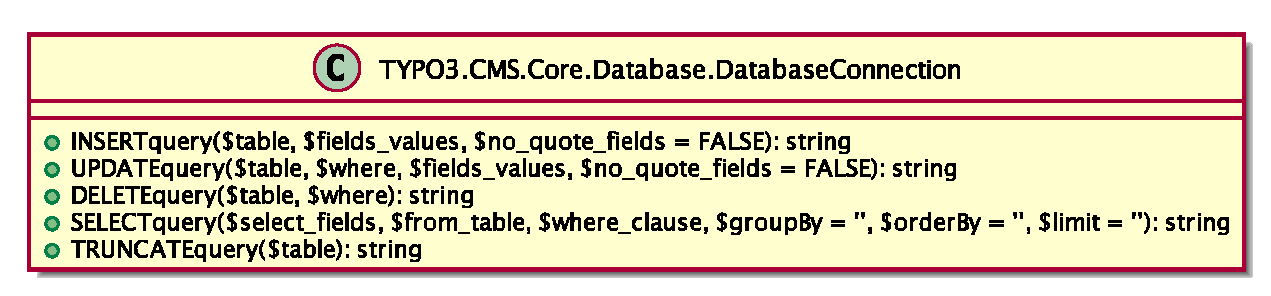
\includegraphics[scale=0.65]{gfx/uml/DatabaseConnectionCreationMethods.eps}
	\caption{DatenbankConnection mit den generierenden Methoden}
	\label{fig:databaseConnectionWithSQLGenerationMethods}
\end{figure}

Folgendes Codebeispiel aus \phpinline{\TYPO3\CMS\Core\Authentication\AbstractUserAuthentication} zeigt die Funktionsweise von \phpinline{SELECTquery()}. Der Kommentar zeigt die generierte SQL-Query.

\begin{listing}
	\begin{phpcode}
// DELETE FROM sys_file_reference WHERE tablenames='pages';
$deleteQuery = $GLOBALS['TYPO3_DB']->DELETEquery(
    'sys_file_reference',
    'tablenames=' . $GLOBALS['TYPO3_DB']->fullQuoteStr('pages', 'sys_file_reference')
);
	\end{phpcode}
	\caption{Löschen eines Datensatzes aus einer Tabelle}
	\label{lst:databaseOldDeleteExample}
\end{listing}

Eine Ebene höher setzt die nächste Gruppe an, die die eben gezeigen Methoden nutzt und den generierten SQL-Query ausführt und eine Ergebnismenge vom Typ \phpinline{mysqli_result} zurückliefert.

\begin{figure}[H]
\centering
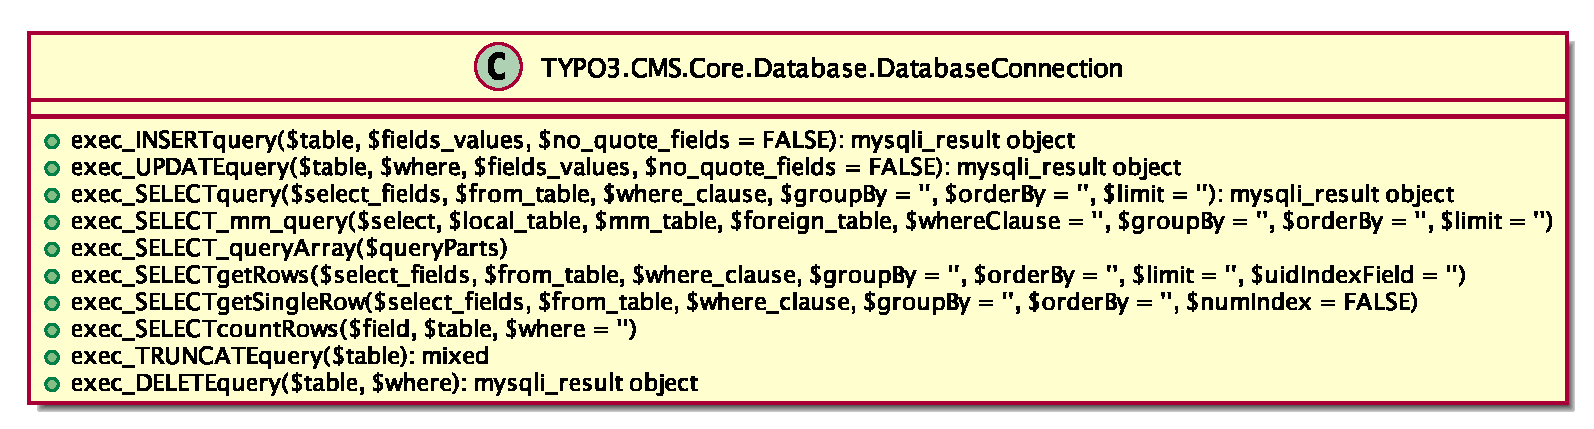
\includegraphics[scale=0.5]{gfx/uml/DatabaseConnectionExecuteMethods.eps}
\caption{DatenbankConnection mit den ausführenden Methoden}
\label{fig:databaseConnectionWithSQLExecutionMethods}
\end{figure}

In der dritte Gruppe befinden sich die Methoden, die im weitesten Sinn zur Verarbeitung der Ergebnismenge genutzt werden. Darunter fallen

\begin{itemize}
	\item jene die die Daten aus der Ergebnismenge extrahieren
	\item mie für die Fehlerbehandlung genutzt werden können,
	\item sowie Methoden die Informationen über die Ergebnismenge breitstellen
\end{itemize}

\begin{figure}[H]
\centering
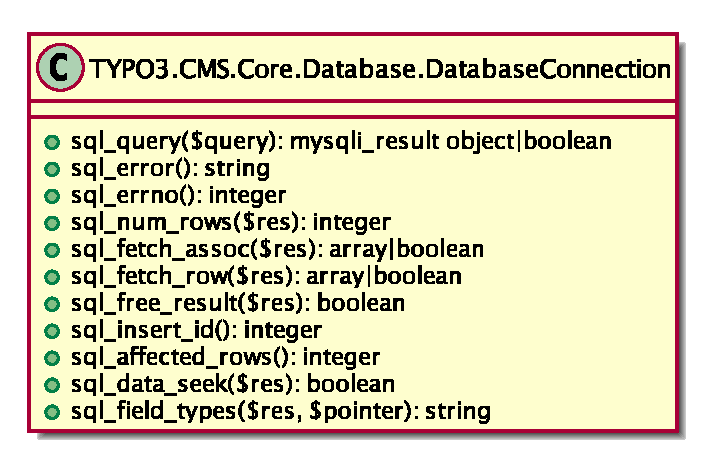
\includegraphics[scale=0.65]{gfx/uml/DatabaseConnectionFetchMethods.eps}
\caption{DatenbankConnection: Methoden zur Verarbeitung der Ergebnismenge}
\label{fig:databaseConnectionWithResultsetsMethods}
\end{figure}

Die nächste Gruppe besteht aus Hilfsmethoden, die genutzt werden um

\begin{itemize}
	\item einen SQL-Query an die Datenbank zu senden
	\item Benutzereingaben zu maskieren
	\item Listen von Integern zu normalisieren
	\item eine \phpinline{WHERE}-Bedingung aus Komma-separierten Datensätzen zu erzeugen
\end{itemize}

\begin{figure}[H]
\centering
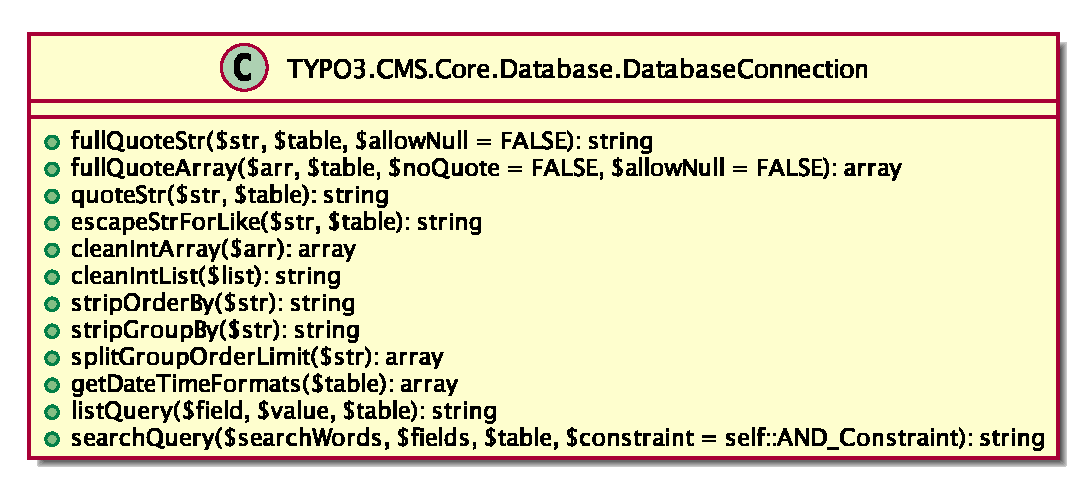
\includegraphics[scale=0.65]{gfx/uml/DatabaseConnectionHelperMethods.eps}
\caption{DatenbankConnection: Hilfsmethoden}
\label{fig:databaseConnectionWithHelperMethods}
\end{figure}

Die letzte Gruppe besteht aus einer Reihe von Methoden, die verschiedene Metadaten über die Datenbank zur Verfügung stellen. Der Name impliziert, dass sie für Administrative Tätigkeiten genutzt werden, was jedoch irreführend ist. Sie werden hauptsächlich während der Installation vom \textit{Installation Tool} verwendet, um Informationen über die zugrundeliegende Datenbank zu erhalten

\begin{figure}[H]
\centering
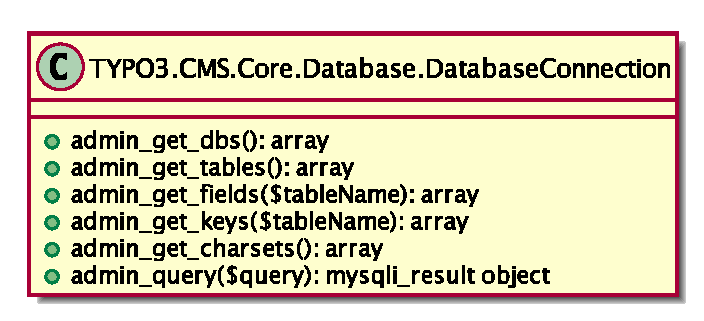
\includegraphics[scale=0.7]{gfx/uml/DatabaseConnectionAdminMethods.eps}
\caption{DatenbankConnection mit administrativen Methoden}
\label{fig:databaseConnectionWithSQLAdminMethods}
\end{figure}

Aus historischen Gründen nutzt die Datenbank API die prozedualen MySQLi Funktionen anstelle der Objekt-orientierten API von MySQLi. Dadurch stellt\\ \phpinline{\TYPO3\CMS\Core\Database\DatabaseConnection} kein Verbindungsobjekt dar - wie zum Beispiel \phpinline{PDO} - sondern eine Sammlung an Datenbankfunktionen. Dadurch gibt es auch kein Objekt, welches die Ergebnismenge repräsentiert, was \phpinline{\TYPO3\CMS\Core\Database\DatabaseConnection} zu einer recht große Klasse mit 1950 Zeilen Code und 76 Methoden.

Im Gegensatz dazu steht die Anzahl von 40 UnitTests mit 49 Assertions für diese Klasse, die lediglich ein paar Hilfsmethoden testen. Es ist somit nicht sichergestellt, ob die Methoden das tun, was sie vorgeben zu tun. In den letzten Monaten wurde jedoch ein Framework für Funktionale Tests in TYPO3 CMS integriert, so dass die Methoden immerhin indirekt getest werden.

[Und dass obwohl TYPO3 CMS mit aktuell 5527 Unit Tests und 8667 Assertions schon eine recht gute Testabdeckung hat 27\% der Dateien und 36\% der abgedeckten Zeilen]

\subsection{Prepared Statements}
\label{currentsituationsubsec:preparedStatements}
Seit TYPO3 CMS 4.5 können Prepared Statements für \mysqlinline{SELECT} Anweisungen verwendet werden. TYPO3 CMS unterstützt sowohl \textit{Posistional Parameters} wie auch \textit{Named Parameters}.

\begin{listing}
\begin{phpcode}
$statement = $GLOBALS['TYPO3_DB']->prepare_SELECTquery(
  '*', 'bugs', 'reported_by = ? AND bug_status = ?'
);
$statement->execute(array('goofy', 'FIXED'));

$statement = $GLOBALS['TYPO3_DB']->prepare_SELECTquery(
  '*', 'bugs', 'reported_by = :nickname AND bug_status = :status'
);
$statement->execute(array(':nickname' => 'goofy', ':status' => 'FIXED'));
\end{phpcode}
\caption{Positional und Named Prepared Statements der TYPO3 CMS Datenbank API}
\label{lst:databaseOldPreparedStatement}
\end{listing}

\phpinline{\TYPO3\CMS\Core\Database\DatabaseConnection::prepare_SELECTquery} liefert ein Objekt der Klasse \phpinline{\TYPO3\CMS\Core\Database\PreparedStatement} zurück, welches sich an der API von \gls{pdo} orientiert.

\begin{figure}[H]
    \centering
    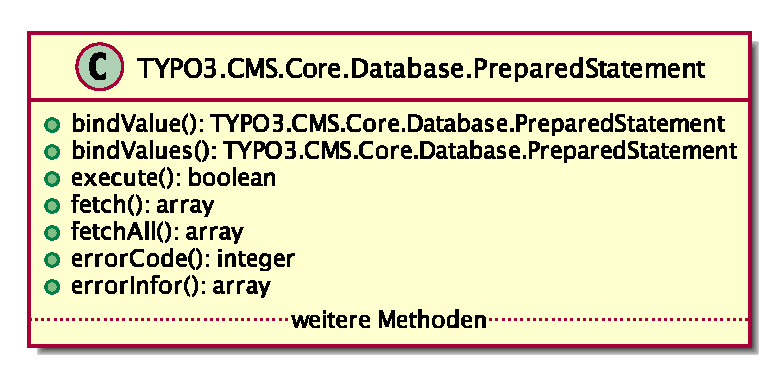
\includegraphics[scale=0.75]{gfx/uml/PreparedStatement.eps}
    \caption{Die Klasse PreparedStatement mit ausgewählen Methoden}
    \label{fig:selectedMethodsOfPreparedStatements}
\end{figure}

\subsection{Datenbankschema}
\label{currentSituation:subsec:databaseSchema}
Nach der Installation von TYPO3 CMS beinhaltet die Datenbank rund 60 einzelne Tabellen. Die Anzahl hängt von der Installation der optionalen Systemextensions ab.

Wichtige Tabellen sind:
\begin{itemize}
	\item pages – Enthält die Seiten
	\item tt\_content – Enthält die Inhaltselement, die auf den Seiten dargestellt werden
	\item be\_groups / fe\_groups – Enhält die Backend- beziehungsweise die Frontendgruppen
	\item be\_users / fe\_users – enthält die Backend- beziehungsweise die Frontendbenutzer
\end{itemize}

Dazu kommen Tabellen
\begin{itemize}
	\item die gecachte Daten und Sessions beinhalten,
	\item die der Indexierung des Inhalts dienen
	\item sowie zum Protokollieren von Systemereignissen
\end{itemize}

Die Inhalte werden in TYPO3 CMS in einer Dateisystem ähnlichen Baumstruktur verwaltet. Eine Webseite wird darin durch einen Datensatz vom Typ \textit{Seite} repräsentiert. Dieser Datensatz hat eine ID, die im gleichnamigen Feld in der Tabelle \texttt{pages} gespeichert wird. Diese ist der \textit{Unique Identifier} des Datensatzes.

Die Inhalte einer Webseite wie Texte, Bilder oder Formulare werden innerhalb einer Seite abgelegt. TYPO3 CMS bietet hierzu eine breite Palette von verschiedenen Elementen an. Zudem können Plugins und wiederum Seiten innerhalb eines Seitendatensatzes abgelegt werden. Diese Liste kann unbegrenzt fortgeführt werden, da jede Extension neue Elemente eingeführen kann, welches in einer Seite ablegbar sind. Es ist lediglich wichtig zu wissen, dass Datensätze innnerhalb von Seiten abgelegt werden können. Die Inhaltselemente werden hauptsächlich in der Tabelle \texttt{tt\_content} gespeichert beziehungsweise in den Tabellen, die die Extension vorsieht.

\begin{figure}[H]
	\centering
	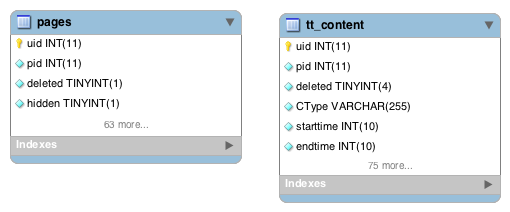
\includegraphics[scale=0.6]{diagrams/DatabasePagesTTContent.png}
	\caption{Die Tabellen pages und tt\_content}
	\label{fig:pagesAndTTContent}
\end{figure}

Die Verknüpfung von Inhaltselement zu übergeordneter Seite erfolgt in der Datenbank über die Spalte \phpinline{pid} (PageID), in der die ID der übergeordneten Seite als Fremdschlüssel gespeichert wird. Listing~\ref{lst:getSubpages} zeigt die SQL-Abfrage, die alle Unterseiten einer Seite zurückgibt. Dabei hat die Seite, dessen Unterseiten abgefragt werden, die \texttt{uid} 4, die in die Abfrage eingesetzt wird. Die Anfrage lautet: Wähle alle Datensätze aus der Tabelle \texttt{pages}, die in der Spalte \texttt{pid} eine 4 stehen haben.

\begin{listing}
	\begin{phpcode}
SELECT * FROM pages WHERE pid=4 ORDER BY sorting
	\end{phpcode}
	\caption{Abrufen von Unterseiten einer Seite}
	\label{lst:getSubpages}
\end{listing}

Analog zum vorigen Listing, zeigt das Folgende die SQL-Anfrage, die alle Inhaltselemente von der Datenbank abfragt.

\begin{listing}
	\begin{phpcode}
SELECT * FROM tt_content WHERE pid=4 ORDER BY sorting
	\end{phpcode}
	\caption{Abrufen von Inhaltselementen einer Seite}
	\label{lst:getContentElements}
\end{listing}

Die beiden Abfragen geben alle Datensätze zurück, was in der Realität jedoch meistens nicht gewünscht ist. Zum Beispiel sollen keine gelöschten Datensätze angezeigt oder nicht alle Inhaltselemente ausgegeben werden. Datensätze werden in der Datenbank nicht gelöscht, sondern in der Spalte \textit{deleted} durch das setzen des Wertes auf 1 als gelöscht markiert. Inhaltselemente werden über die Spalte \texttt{CType} nach ihrem Typ gefiltert. Um das gewünschte Ergebnis zu erhalten müssen \mysqlinline{WHERE}-Klauseln formuliert werden, was die doch recht trivialen SQL-Anfragen schnell komplex werden lässt.

In TYPO3 CMS können die Benutzerrechte sehr granular eingestellt werden. Die Einstellungen können per Benutzer oder Benutzergruppe vorgenommen werden.
Dabei kann ein Benutzer Mitglied keiner, einer oder mehrerer Benutzergruppen sein. Zudem kann eine Benutzergruppe keinen, einen oder mehrere Benutzer enthalten. Dies stellt eine Many-to-Many-Relation dar.

In der Datenbank wird die Zugehörigkeit von Benutzer <-> Gruppe von den Tabellen \texttt{fe\_users} und \texttt{fe\_groups} beziehungweise \texttt{be\_users} und \texttt{be\_groups} abgebildet.

\begin{figure}[H]
	\centering
	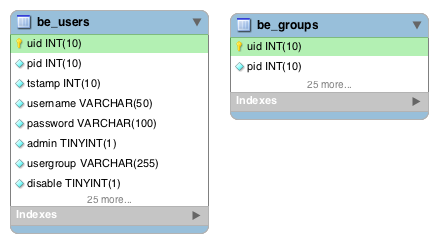
\includegraphics[scale=0.6]{diagrams/DatabaseBEUserGroup.png}
	\caption{Die Tabellen be\_users und be\_groups}
	\label{fig:beUsersAndBeGroups}
\end{figure}

Hier fällt der Datentyp der Spalte \texttt{usergroup} auf, die ID der Gruppe des Benutzers speichert. Hier ist ein \mysqlinline{VARCHAR} definiert, obwohl die Spalte \texttt{uid} den Typ \mysqlinline{INT} hat. Dies liegt darin, dass die Zuordnung der Benutzer zu Gruppe über eine kommaseparierte Liste erfolgt:

\begin{Verbatim}[samepage=true]
+----+-----+------------+----------+----------+-------+-----------+---------+--------+---------+
| id | pid |   tstamp   | username | password | admin | usergroup | disable | hidden | deleted |
+----+-----+------------+----------+----------+-------+-----------+---------+--------+---------+
|  1 |  0  | 1191353353 | admin    |  secret  |   1   |           |    0    |   0    |    0    |
|  2 |  0  | 1281556682 | snape    |  secret  |   1   |    43     |    0    |   0    |    0    |
|  3 |  0  | 1191353353 | hagrid   |  secret  |   0   |  5,32,43  |    0    |   1    |    0    |
+----+-----+------------+----------+----------+-------+-----------+---------+--------+---------+
\end{Verbatim}

Diese stellt lediglich ein Beispiel dar. Kommaseparierte Listen gibt es an vielen Stellen in der Datenbank. Die API von TYPO3 CMS stellt Methoden bereit, die die Liste für die weitere Verabreitung aufbereiten.

Dieses Konstrukt existiert wahrscheinlich seit Beginn des Systems und es ist zu vermuten, dass damit eine Many-to-Many-Tabelle vermieden werden sollte, was die Komplexität der SQL-Anfrage erhöht.

Um die kommaseparierten Listen aufzulösen, müßte eine weitere Tabelle eingeführt werden, dessen zwei Spalten jeweils auf die \texttt{id} der beiden zu verknüfenden Tabellen referenzieren.

\begin{figure}[H]
	\centering
	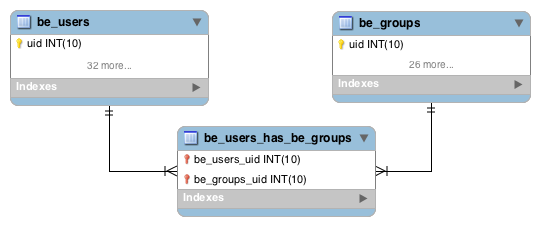
\includegraphics[scale=0.6]{diagrams/DatabaseBEUserGroupMM.png}
	\caption{Normalisierung über Many-to-Many Tabelle}
	\label{fig:beUsersHasBeGroups}
\end{figure}

\begin{Verbatim}[samepage=true]
+--------------+---------------+
| be_users_uid | be_groups_uid |
+--------------+---------------+
|      2       |      34       |
|      3       |       5       |
|      3       |      32       |
|      3       |      43       |
+--------------+---------------+
\end{Verbatim}

TYPO3 CMS nutzt weder Datenbankseitige \textit{Constraints} noch Fremdschlüssel Definitionen. Alle Referenzierungen werden von TYPO3 CMS selbst verwaltet.

		%-----------------------------------------------
% Dateiname: Protype.tex
% Autor    : Stefano Kowalke <blueduck@gmx.net>
% Lizenz   : BSD
%-----------------------------------------------
\chapter{Prototypischer Nachweis der Herstellbarkeit}
\label{ch:protoype}

\section{Refactoring der alten Datenbank API}
\subsection{Tests für die alte Datenbank API}

\section{Testgetriebene Implementierung der neuen Datenbank API}
- Adapter
- alte API Klasse erbt von neuer API Klasse
- Verbindung mit der Datenbank via Doctrine
- Methodenübername wenn sinnvoll
- Neue Methoden

\subsection{Einführung von Query Objekten}
\subsubsection{SELECT}
\subsubsection{INSERT}
\subsubsection{UPDATE}
\subsubsection{DELETE}
\subsubsection{TRUNCATE}

\section{Anwendung der neuen Datenbank API}
%\subsection{Anpassungen an TYPO3}
\section{Überprüfen der Funktionalität}

		%%-----------------------------------------------
% Dateiname: Outlook.tex
% Autor    : Stefano Kowalke <blueduck@gmx.net>
% Lizenz   : BSD
%-----------------------------------------------
\chapter{Ausblick}
\label{ch:outlook}
\begin{itemize}
	\item{Einladung zum ACME14N}
	\item{Einbau in den Core}
	\item{Nutzung von Doctrine Migrations}
	\item{Nutzung von Doctrine ORM}
	\item{Umbau der Datenbankobjekts zu einem Datenbankconnection Pool}
	Design Pattern Static Fabric oder Fabric
\end{itemize}

	\backmatter
		%-----------------------------------------------
% Dateiname: Conclusion.tex
% Autor    : Stefano Kowalke <blueduck@gmx.net>
% Lizenz   : BSD
%-----------------------------------------------
\chapter{Zusammenfassung}
\label{ch:conclusion}

	\appendix
		\printbibliography[title={Quellenverzeichnis}]
		\includepdfset{pagecommand={\thispagestyle{headings}}}
		% Print glossar
		\printglossary[type=main,title=Glossar,toctitle=Glossar,style=altlist]
		% Print Akronyms
		\printglossary[type=\acronymtype, title=Abkürzungsverzeichnis,toctitle=Abk\"urzungsverzeichnis,style=long]% Der Umlaut muß hier so angegeben werden, da es sonst Anzeigeprobleme im PDF-Viewer gibt.
		\listoftables
		\listoffigures
		\listoflistings
		\includepdf[pages={1,2}, addtotoc={1,chapter,0,Tabelle alte API Methoden - neue Methoden,chap:int},  scale=0.9]{Bib/Functions.pdf}
		%-----------------------------------------------
% Dateiname: Statement.tex
% Autor    : Stefano Kowalke <blueduck@gmx.net>
% Lizenz   : BSD
%-----------------------------------------------
\chapter{Eidesstattliche Erkl\"arung}
\label{ch:erklaerung}

Hiermit versichere ich, die vorliegende Arbeit selbstständig und unter
ausschließlicher Verwendung der angegebenen Literatur und Hilfsmittel erstellt zu haben.
\vspace*{2em}
\\
\myLocation, den \today \\\\

\underline{\ \ \ \ \ \ \ \ \ \ \ \ \ \ \ \ \ \ \ \ \ \ \ \ \ \ \ \ }\\\\
\small{\myName}

		% Glossaries und Akronyme kommen hier hin oder ins Frontmatter
\end{document}
